\vspace{-10ex}%
\rule{\textwidth}{0.3pt}
\vspace{10ex}

\emph{
This chapter will guide the reader through the whole process of developing a system prototype. Designing the PCB, soldering the components, troubleshooting the board and writing the necessary code are some of the steps involved and they will all be described in detail here.
}

\section{Schematics}
The schematics over the circuit is created by placing all the components discussed earlier, every IC have a small number of components that are placed in a way so that it is easy to understand which components belong to which. A title is added to every part in the design for a good overview of the system. Since the section which included the radio is large it is placed on a separate page. When additional components are added in additional pages can be inserted. These schematics can be found in \autoref{appendix_schematics}.

\section{Layout} 
\subsection{First design} The first of two boards is 3.5 times 3.5 mm in size. The different parts of the circuit are laid out in a way that it is easy to inspect and resolder if necessary. The main components of the board are placed close to each other at one side to get an idea of the design for the final product. This board is equipped with some test points for easy connections with test probes and oscilloscope. The silkscreen print on the top of the board was vague at some places and made distinguish them from each other hard. The pin one location at one part could not be spotted.  A view of the board can be seen in \autoref{PCB_rev1}. 

\begin{figure}[H]
	\centering
    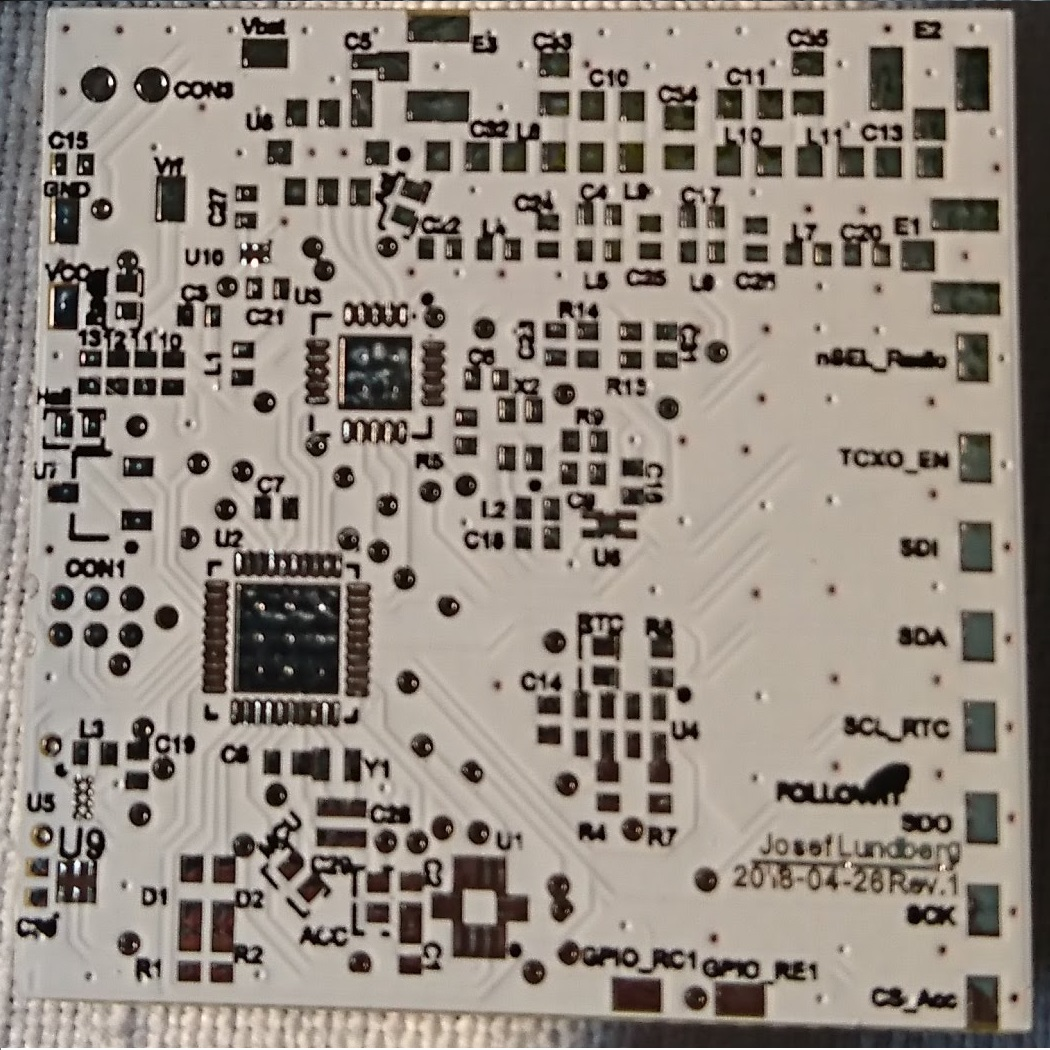
\includegraphics[width=.8\linewidth]{Figures/PWB}
	\captionsource{First (1) revision circuit board.}{Author}
	\label{fig:pcbr1}
\end{figure}

\section{Communication}

\subsection{UART}
The \gls{uart} connection interfered with another connection which leads to one function not working as intended. The function that is the enabling line to the \gls{ldo} which powers the oscillator for the radio. It is fixed by connection one of the extra pins that was laid out beforehand directly to the \gls{ldo}. The transmitting half of the \gls{uart} connection is working as intended on this version, some of the resulting data which is sent to the computer can be seen in \autoref{fig:uart_first_rev}.

\begin{figure}[H] 
    \centering 
    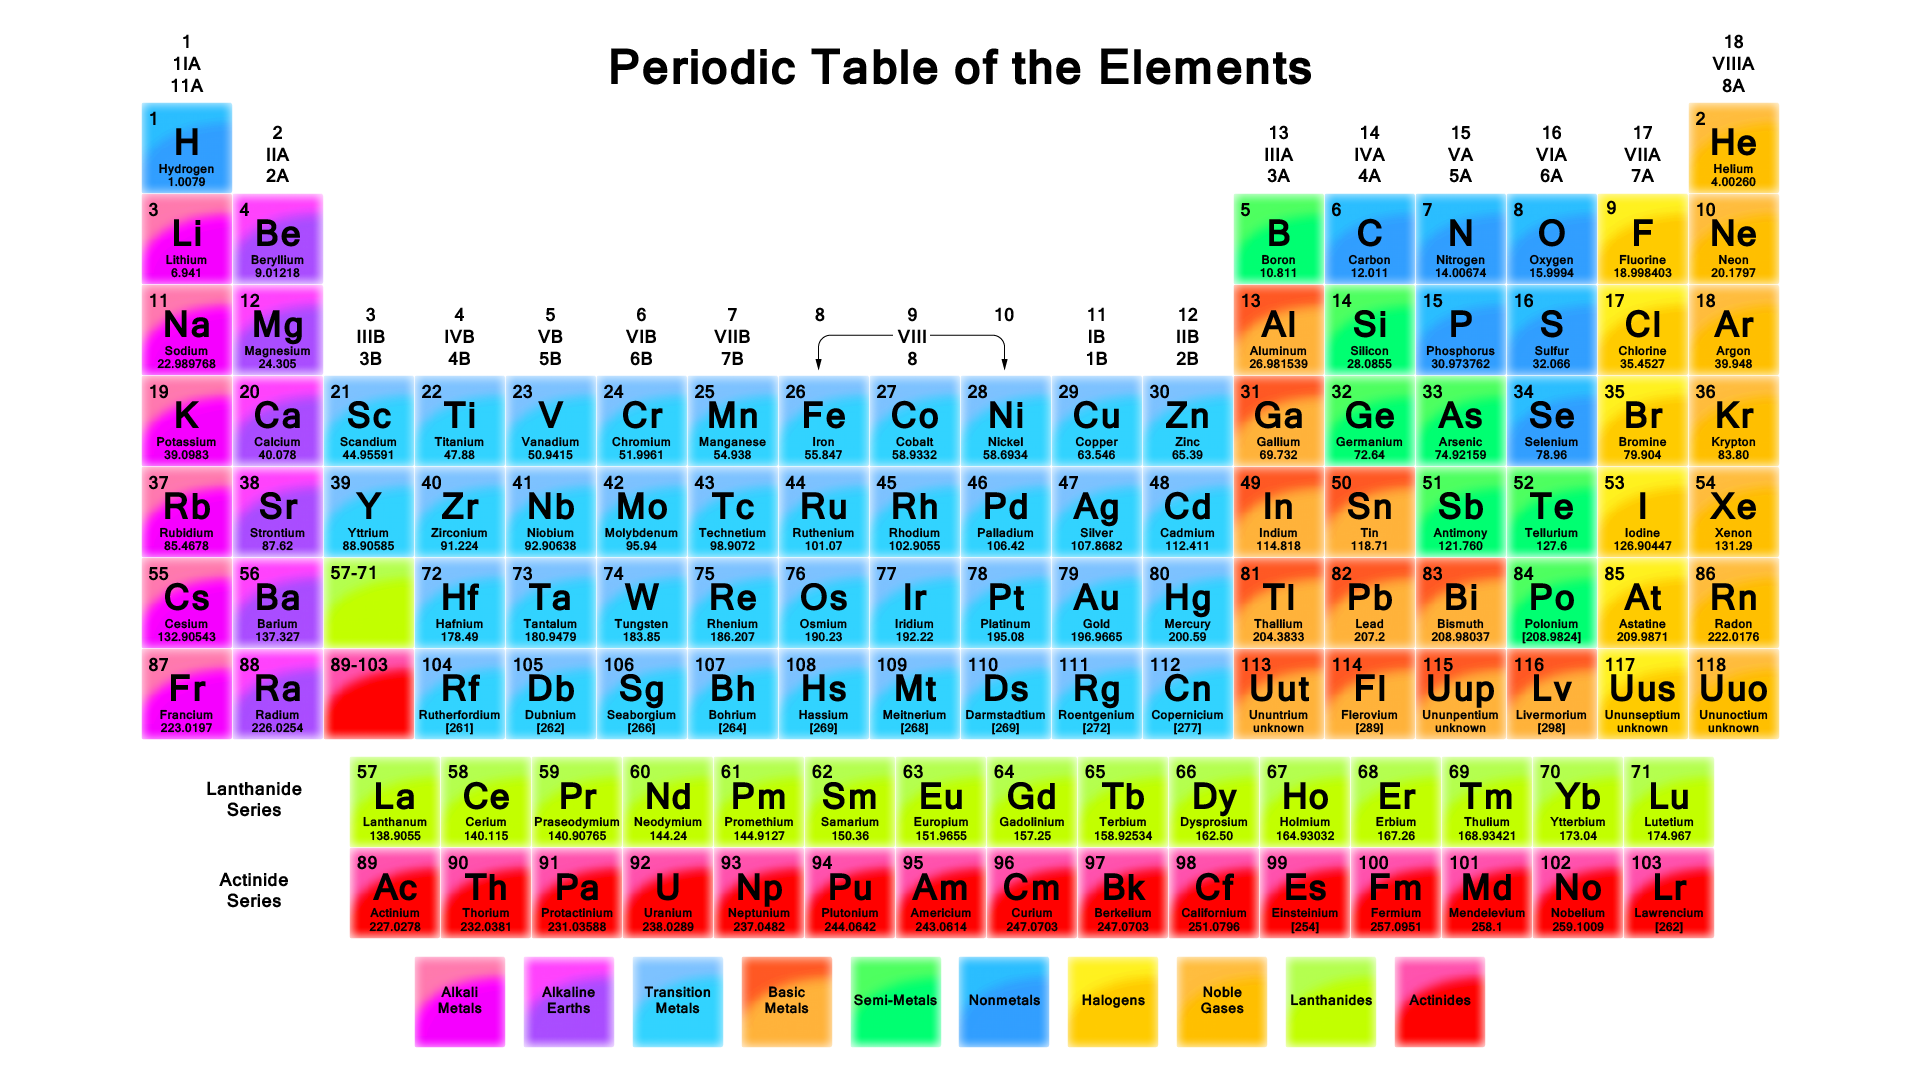
\includegraphics[width=.8\linewidth]{Figures/uart_first_rev} 
    \captionsource{Simple \gls{uart} transmission to a \gls{pc}}{Aurthor}
    \label{fig:uart_first_rev} 
\end{figure} 

\subsection{SPI}
Testing started with both the\gls{mcu}, radio and accelerometer soldered to the board. No communications were achieved when both of these slave devices were connected at the same time. After some troubleshooting, the failing factor of this is the accelerometer having it's \gls{spi} connection the other way around. The data out (SDO) line was connected to the data output, and the SDI was connected to the data input line of the accelerometer.  


\section{improvements}
From the first version some valuable point can be determined, both for the layout, schematics, and wiring.









% Kanske inte
\begin{comment}
\section{Power consumption}
When running the processor at operation speed and voltage the 
The power consumption is first mesured with only the processor connected. 
\end{comment}